\documentclass{article}

\usepackage{fancyhdr}
\usepackage{extramarks}
\usepackage{amsmath}
\usepackage{amsthm}
\usepackage{amsfonts}
\usepackage{tikz}
\usepackage[plain]{algorithm}
\usepackage{algpseudocode}
\usepackage{enumerate}
\usepackage{mathtools}
\usepackage{forest}
\usepackage{adjustbox}
\usepackage[table]{colortbl}
\usepackage{graphicx}
\graphicspath{ {images/} }

\usetikzlibrary{automata,positioning}

%
% Basic Document Settings
%

\topmargin=-0.45in
\evensidemargin=0in
\oddsidemargin=0in
\textwidth=6.5in
\textheight=9.0in
\headsep=0.25in

\linespread{1.1}

\pagestyle{fancy}
\lhead{\hmwkAuthorName}
\chead{\hmwkClass\ (\hmwkClassInstructor\ \hmwkClassTime): \hmwkTitle}
\rhead{\firstxmark}
\lfoot{\lastxmark}
\cfoot{\thepage}

\renewcommand\headrulewidth{0.4pt}
\renewcommand\footrulewidth{0.4pt}

\setlength\parindent{0pt}

%
% Create Problem Sections
%

\newcommand{\enterProblemHeader}[1]{
    \nobreak\extramarks{}{Problem \arabic{#1} continued on next page\ldots}\nobreak{}
    \nobreak\extramarks{Problem \arabic{#1} (continued)}{Problem \arabic{#1} continued on next page\ldots}\nobreak{}
}

\newcommand{\exitProblemHeader}[1]{
    \nobreak\extramarks{Problem \arabic{#1} (continued)}{Problem \arabic{#1} continued on next page\ldots}\nobreak{}
    \stepcounter{#1}
    \nobreak\extramarks{Problem \arabic{#1}}{}\nobreak{}
}

\setcounter{secnumdepth}{0}
\newcounter{partCounter}
\newcounter{homeworkProblemCounter}
\setcounter{homeworkProblemCounter}{1}
\nobreak\extramarks{Problem \arabic{homeworkProblemCounter}}{}\nobreak{}

%
% Homework Problem Environment
%
% This environment takes an optional argument. When given, it will adjust the
% problem counter. This is useful for when the problems given for your
% assignment aren't sequential. See the last 3 problems of this template for an
% example.
%
\newenvironment{homeworkProblem}[1][-1]{
    \ifnum#1>0
        \setcounter{homeworkProblemCounter}{#1}
    \fi
        \section{Problem \arabic{homeworkProblemCounter}}
    \setcounter{partCounter}{1}
    \enterProblemHeader{homeworkProblemCounter}
}{
    \exitProblemHeader{homeworkProblemCounter}
}

%
% Homework Details
%   - Title
%   - Due date
%   - Class
%   - Section/Time
%   - Instructor
%   - Author
%

\newcommand{\hmwkTitle}{Homework \#8}
\newcommand{\hmwkDueDate}{April 14, 2016}
\newcommand{\hmwkClass}{CS 373}
\newcommand{\hmwkClassInstructor}{Professor David Garrison}
\newcommand{\hmwkClassTime}{Section B1}
\newcommand{\hmwkAuthorName}{Tim Hung}

%
% Title Page
%

\title{
    \vspace{2in}
    \textmd{\textbf{\hmwkClass:\ \hmwkTitle}}\\
    \normalsize\vspace{0.1in}\small{Due\ on\ \hmwkDueDate\ at 2:20pm}\\
    \vspace{0.1in}\large{\textit{\hmwkClassInstructor\ \hmwkClassTime}}\\
}

\author{\textbf{\hmwkAuthorName}}
\date{}

\renewcommand{\part}[1]{\textbf{\large Part \Alph{partCounter}}\stepcounter{partCounter}\\}

%
% Various Helper Commands
%

% Useful for algorithms
\newcommand{\alg}[1]{\textsc{\bfseries \footnotesize #1}}

% For derivatives
\newcommand{\deriv}[1]{\frac{\mathrm{d}}{\mathrm{d}x} (#1)}

% For partial derivatives
\newcommand{\pderiv}[2]{\frac{\partial}{\partial #1} (#2)}

% Integral dx
\newcommand{\dx}{\mathrm{d}x}

% Alias for the Solution section header
\newcommand{\solution}{\textbf{\large Solution}}

% Probability commands: Expectation, Variance, Covariance, Bias
\newcommand{\E}{\mathrm{E}}
\newcommand{\Var}{\mathrm{Var}}
\newcommand{\Cov}{\mathrm{Cov}}
\newcommand{\Bias}{\mathrm{Bias}}

\begin{document}

\maketitle

\pagebreak

\begin{homeworkProblem} 

    \begin{figure}
        \centering
        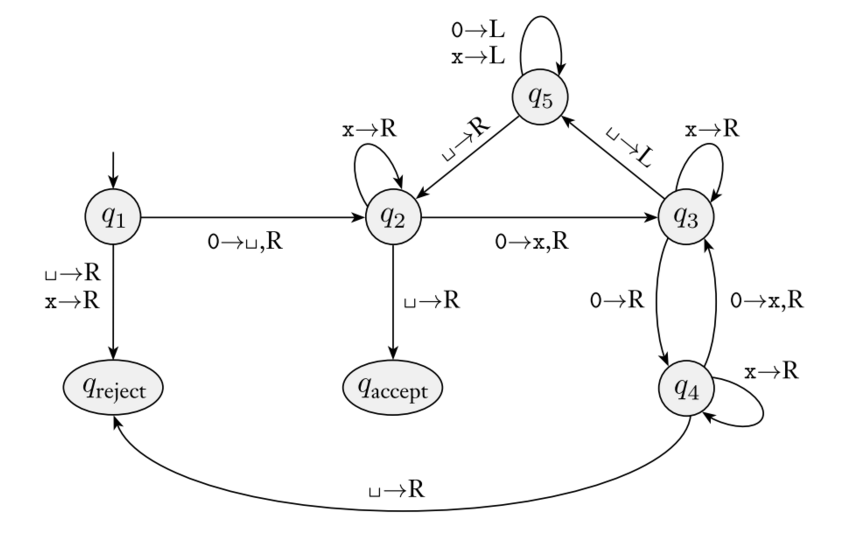
\includegraphics[width=\textwidth]{TM_M2}
        \caption{State diagram for Turing machine $M_2$}
    \end{figure}

    \textbf{(a)}    Give the sequence of configurations that $M_2$ enters when started on the input string '0'.
    \[
        q_1 0 
        \Rightarrow \sqcup q_2 \sqcup 
        \Rightarrow \sqcup \sqcup q_{\text{accept}}
    \]
    
    \textbf{(c)}    Give the sequence of configurations that $M_2$ enters when started on the input string '000'.
    \[
        q_1 000
        \Rightarrow \sqcup q_2 00
        \Rightarrow \sqcup xq_30
        \Rightarrow \sqcup x0q_4\sqcup
        \Rightarrow \sqcup x0\sqcup q_{\text{reject}}
    \]
\end{homeworkProblem}

\pagebreak

\begin{homeworkProblem} 
    \begin{figure}
        \centering
        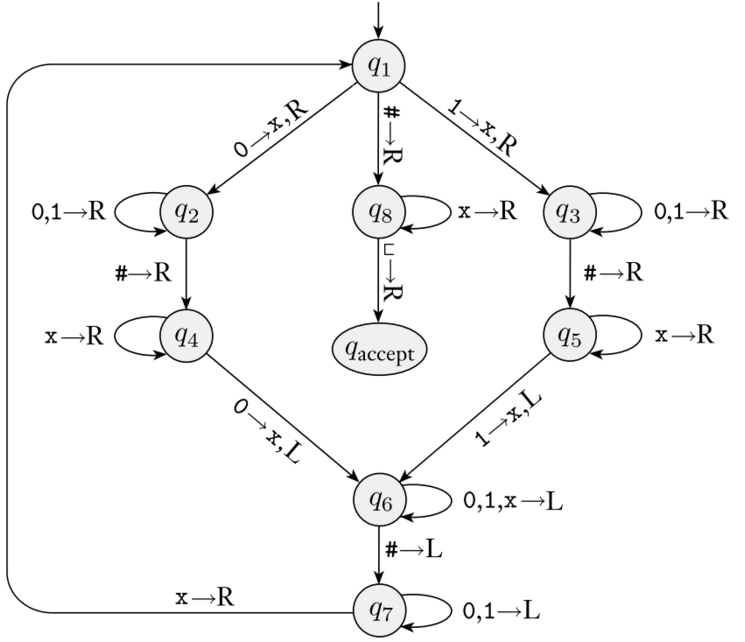
\includegraphics[width=\textwidth]{TM_M1}
        \caption{State diagram for Turing machine $M_1$}
    \end{figure}
    \textbf{(b)}    Give the sequence of configurations that $M_1$ enters when started on the input string '1\#1'.
    \[
        q_11\#1
    \]

    \textbf{(c)}    Give the sequence of configurations that $M_1$ enters when started on the input string '1\#\#1'.
    \[
        q_11\#\#1
        \sqcup q_3\#\#1
        \sqcup\#q_5\#1
        \sqcup\#\#q_{\text{reject}}1
    \]

\end{homeworkProblem}

\pagebreak

\begin{homeworkProblem} 
    Describe a Turing machine, sequence of steps, that recognizes $\{w|w\in{a, b, c}*$ such that the number of a's in w $<$ the number of b's in w and the number of a's in w = the number of c's in w $\}$.

    \textbf{Solution}
    \begin{figure}[here]
        \centering
        \begin{tikzpicture}[shorten >=1pt,node distance=2cm,on grid,auto]
            \node[state] (q_1) {$q_1$};
            \node[state] (q_2) [right=of q_1]{$q_2$};

            \path [->] 
                (q_1) 
                    edge node{0} (q_2);

        \end{tikzpicture}
        \caption{This sure is a graph right here yes it is.}
        \label{fig:multiple5}
    \end{figure}
        
\end{homeworkProblem}

\begin{homeworkProblem} 
    A 2-PDA is a PDA with two stacks. In this problem we want to kind of show that a 2-PDA is as
    powerful as a Turing machine. To do this, show the equivalent transitions for a 2-PDA for the
    Turing machine transitions (qi, X) -> (qj, A, L) and (qi, X) -> (qj, A, R) (in state qi read X, write A,
    and move left or right and transition to state qj). The transitions for a 2-PDA are of the form (qi,
    X, S1, S2) -> (qj, T1, T2) (in state qi, read X, pop S1 from stack 1, pop S2 from stack 2, transition to
    state qj, push T1 onto stack 1 and push T2 onto stack 2). You don't have to prove the transitions
    are equivalent, just tell me what they are.

    In this problem we want the 2-PDAs first stack to represent the contents of the tape to the left of
    the Turing machine's read/write head and the second stack to represent the contents of the
    tape under the Turing machine's read/write head and to the right of the read/write head. Once
    we visualize it this way, it should be fairly obvious that a 2-PDA can accept any language that a
    Turing machine can as long as we can duplicate the two Turing machine transitions (left move
    and right move).

    To correctly initialize the second stack of the 2-PDA we simply read the input and push it into
    the first stack and then pop everything out of the first stack while pushing onto the second
    stack. Once we have done this, the first stack is empty and the second stack contains the input
    in the correct order.
\end{homeworkProblem}

\begin{homeworkProblem}
    Give implementation-level descriptions of Turing machines that decide the follow language:
    \[
        \{w|w\in\{0,1\}\text{ and does not contain twice as many 0s as 1s}\}
    \]
\end{homeworkProblem}

\begin{homeworkProblem}
    Prove the class of Turing recognizable languages is closed under the union operation (construction and proof).
\end{homeworkProblem}

\begin{homeworkProblem}
    Prove the class of decidable languages is closed under concatenation (construction and proof)
\end{homeworkProblem}

\begin{homeworkProblem}
    Prove the class of decidable languages is closed under intersection (construction and proof)
\end{homeworkProblem}

\begin{homeworkProblem}
    Prove the class of Turing recognizable languages is closed under the star operation (construction and proof)
\end{homeworkProblem}

\begin{homeworkProblem}
    Show that a language is decidable if and only if some enumerator enumerates the language in the standard string order.
\end{homeworkProblem}

\pagebreak

\begin{homeworkProblem}
(10 points) Enumerate the nodes in the following graph in (a) BFS order and (b) DFS order, starting from node 1. 
\begin{figure}[here]
    \centering
    \begin{tikzpicture}[shorten >=1pt,node distance=2cm,on grid,auto]
        \node[shape=circle,draw=black] (1) at (2,2)    {$1$};
        \node[shape=circle,draw=black] (2) at (.5,1)   {$2$};
        \node[shape=circle,draw=black] (3) at (2,1)    {$3$};
        \node[shape=circle,draw=black] (4) at (3.5,1)  {$4$};
        \node[shape=circle,draw=black] (5) at (0,0)    {$5$};
        \node[shape=circle,draw=black] (6) at (1,0)   {$6$};
        \node[shape=circle,draw=black] (7) at (2,0)    {$7$};

        \path [->] (1) edge (2);
        \path [->] (1) edge (3);
        \path [->] (1) edge (4);
        \path [->] (2) edge (5);
        \path [->] (2) edge (6);
        \path [->] (3) edge (7);

    \end{tikzpicture}
    \caption{This sure is a graph right here yes it is.}
    \label{fig:multiple5}
\end{figure}

\textbf{Solution}
    \begin{enumerate}[a)]
        \item
            BFS: 1, 2, 3, 4, 5, 6, 7
        \item  
            DFS: 1, 2, 5, 6, 3, 7, 4
    \end{enumerate}
\end{homeworkProblem}

\end{document}
